%%%%!!!!!!!!!!!!!!!!!!!!! todo
% check value of distance and corresponding SNR
% In the future, ene could set a dynamic criteria of pulse width  with distance, according to the trigger model and pulse width in use..

% trigger mode discussion
%%%%%%%%%%%%%%%%%%%%%%%%%%%%%%%%%%%%%%%%%%%%%

\chapter{Time Discrimination-ADC}\label{ch:ADC_BM}
\section{Problem Description}
In addition to the TDC-based approaches, we can also use ADC. The ADC-based time discrimination is using ADC to convert analog signals output from a detector to digital signals, and measure the time of the digital returning pulse. The structure of the ADC-based discriminator is shown in Figure~\ref{fig:schematic_ADC}. The time discrimination can be achieved by applying digital versions of the TDC-based timing algorithms to the digital signals, or by taking advantages of the shape information contained in the digital signals.
\subsection{Digital version of the analog timing techniques}
 The digital versions of the TDC-based timing algorithms include the aforementioned algorithms like leading-edge detection techniques and CFDs. The details of those methods are described in the above sections and are skipped here, but one should notice some drawbacks of the digital version algorithms. One is that for the digital signals, the threshold generally does not coincide to the sample points of the signal. Therefore, interpolation between neighborhood samples is needed to find the exact time mark corresponding to the threshold value. Linear interpolation is a common selection, but the interpolation could affect the timing accuracy, depending on the local linearity of the signal. More specifically, if the curvature of a signal in the proximity of the threshold is large (the pulse has a nonlinear shape), time walk could occur. Note that this walk error is different than the walk error mentioned in the TDC-based approaches. The effect of the curvature is illustrated in Fig \todo{(Fig10.27 Mahammad book). }
\subsection{Detector and Estimator}
% The digital version of the TDC-based techniques utilizes the ADC as a TDC, which limits the potential of the ADC since the valuable shape information contained in the digital signal is not taken into consideration which could improve the accuracy of signal detection and estimation. Therefore, we proposed the time discrimination algorithms that take advantage the shape information and are generally composed of a detector and an estimator. The detector is to take the digital signal output from an ADC and determine the presence or absence of a predefined signal from a signal contaminated by noise. In our case, that is if a Gaussian pulse with certain characteristics (\ie rise time, pulse width, \etc) is present in the returning signal. The absence or presence of a return pulse is denoted by a binary hypothesis test $\mathcal{H}_1$: pulse or $\mathcal{H}_0$: noise.Subsequently, if the pulse is present, an estimator is needed to estimate the values of the parameters of the signal (the arrival time of return pulses in our case). \\
% In this section, we first introduce the fundamentals of the ADC, followed by two algorithms that determines the presence of a return signal and estimates the arrival time of the return pulse.




%%


%% + literature review of detectors and estimators: peak, LSE, MF ...
% \subsubsection{Estimator}
% Many different estimators are available for extraction of signal parameters, \eg the arrival time of a signal, ranging from the simple peak estimator(PE) and time-over-threshold estimator by averaging the detection of the leading and falling edge of a signal, to more advanced Maximum Likelihood Estimator(MLE) and Least Square Estimator(LSE). This work will focus on the PE, MLE, and LSE.The theory will be introduced, followed by the implementation of the estimators to synthetic and real signals.

% \subsubsection{Peak Estimator}
% The PE is straightforward and efficient and has been widely applied to time-of-flight determination and object recognition using lidar and ultrasonic sensors measurements\cite{Steinvall2000EffectsSections,Steinvall2001Three-dimensionalModeling,Steinvall2007,Steinvall2005RangeRadars,Der1997SimulationMeasurements,Gronwall2006GroundApplications,richmond2010direct,Anitha2011Time-of-FlightTechniques}.The peak estimator is either used directly on the raw analog signal or followed by a matched filter and estimate the peak of the convolution result\cite{Der1997SimulationMeasurements}.


 
% \subsection{Maximum Likelihood Estimator} \label{sec:MLE}
% MLE is widely used, 
% papers: steinvall2005range (fit to gaussian), Buschelman, Joly, petrick, tomi



The digital version of the analog timing techniques that utilize the ADC as a TDC limits the potential of the ADC because the shape information of the digital signal which is valuable to improve the accuracy of signal detection and estimation is ignored. In this section, the time discrimination algorithms that capture the characteristics of the pulse are introduced, which is called ADC-based algorithms. The ADC-based timing algorithms are generally composed of a detector and an estimator. The function of the detector is to take the signal collected by an ADC and determine the presence or absence of a predefined signal from the raw signal contaminated by noise. If a pulse is detected, an estimator is needed to estimate the values of the parameters of the signal by mathematically modeling the signal. In our case, the detector is to determine if a return pulse with certain characteristics (\ie shape, rise time, and pulse width, \etc) exists in the collected signal, and estimate the arrival time of the pulse if it is present. In this section, we will focus on two detection and estimation algorithms: centroid-based detection and estimation algorithm(centroid-method) and Neyman-Pearson(NP) detector (or Matched filter). The principle of the algorithms will be illustrated first followed by the application of the algorithms to simulated signals and/or signals collected from real experiments. The centroid detector will be introduced in this section and the Matched filter will be introduced in Chapter~\ref{ch:NP}.

\subsection{Data pre-processing}
To reduce the deterioration of the outliers on the detection algorithms, the digital signals are filtered by a median filter with a kernel with a size of 3 or 5. Small size of kernels were used to avoid distortion of the signal due to the filter. Examples of the signals before and after filtering are shown in \todo{Figure}. The median filter efficiently removes the sparse random outliers, but not the effect is not obvious on frequently occurring noises. %add median filter%

% %
%  Bench-mark detection
% %
\section{Benchmark Detection and Estimation}
\subsection{Metrics for signal detection}\label{sec:bm_metrics}
In the benchmark detection, two metrics are utilized for the hypothesis determination of a return signal. The metrics include the number of points of a signal above the ADC threshold and the pulse width of the signal. In this section, the metrics and the corresponding criterion are defined first, followed by an introduction of the algorithm used for the pulse width calculation.
\subsubsection{Metric 1: Number of points above threshold}
Strong random noises could false-trigger an ADC, but it is very unlikely a large number of consecutive data points of the random noise could excess the threshold. In this case, we use the number of data points of a signal above the ADC threshold (\abbr number above threshold or NaT) as the first metric to distinguish the false-triggering induced by random noise. Usually, the ADC threshold is set at a constant value (\ie 3x noise floor), so when the amplitude of a signal changes, the NaT varies in a range according to the target distance, and stronger signals have a larger value of NaT. To make the metric applicable to signals from different distances, a range of the NaT is defined, and the upper and lower bound of the range is determined by measuring the NaT of noise-free return signals from the shortest and furthest distance studied in this work, specifically, $2~m$ and $300~m$. The corresponding SNRs are $60~dB$ and $8~dB$ and the measured NaTs are 52 points and 10 points, respectively. Therefore, when the ADC receives a signal the NaT of a return signal is counted first, and if the NaT exceeds the range of 10 and 52, the signal is considered to be $\hzero$.
% Metric 2: pulse width
\subsubsection{Metric 2: Pulse width}
Usually, the pulse width of a signal remains constant through the whole signal propagation, assuming negligible distortion of the pulse shape due to the reflection by molecules in the atmosphere and the response time of electrical systems. In this case, we can determine the hypothesis of a return signal by comparing its pulse width with the one of the transmit pulse. The expression of the pulse width of a signal can be derived from Equation \eqref{eq:pw}, such that
\begin{equation} \label{eq:bm_pw}
    \Delta t_w = \frac{E}{P_{r, peak}},
\end{equation}
assuming the approximation for the pulse energy mentioned in Section~\ref{sec:pw} also holds for digital signals. Theoretically, the energy of a signal can be obtained by integrating the signal over an infinitely long time duration, while in practice the signal is truncated due to a finite number of points that can be collected by an ADC. Similar to Metric 1, to determine the criteria, the pulse width of noise-free signals from the shortest and furthest distance was calculated using the method that will be introduced in Section~\ref{sec:bm_pw_cal}. The measured pulse width ranges from $4.91~ns$ (SNR is $8~dB$) to $5.42~ns$ (SNR is $60~dB$), and the variation of the pulse width from the mean value is $0.51~ns$ or $10\%$ of the mean. Therefore, a tolerance of the measured pulse width is defined, such that if the difference between the measured pulse width $\Delta t_{w,meas}$ and the reference pulse width $\Delta t_{w,ref}$ is smaller than $10\%$ of the reference, the signal passes Metric 2. In this study, the reference pulse width is $5.17~ns$. Mathematically, we claim the signal passes Metric 2 if
\begin{equation}\label{eq:bm_cri2}
    |\Delta t_{w, meas} - \Delta t_{w,ref}| < 10\%\Delta t_{w,ref}
\end{equation}\par
\subsubsection{Signal detection}
After defining the metric and the corresponding criterion, we can follow the flowchart shown in Figure~\ref{fig:bm_flowchart} to determine the hypothesis of a return signal. In the detection process, the counting of NaT is straightforward, but the pulse width needs to be calculated from the signal which will be illustrated next.
\begin{figure}[htb] % position options
\centering
\graphicspath{ {figures/} }
\includegraphics[width=0.5\textwidth]{figures/chapter6_ADC/BM_flowchart.png}
\caption{Flow chart of benchmark detection algorithm}
\label{fig:bm_flowchart}
\end{figure}
% pulse width calculation
\subsection{Pulse width calculation} \label{sec:bm_pw_cal}
According to Equation \eqref{eq:bm_pw}, we need to obtain the energy and the peak power of a signal before calculating the pulse width. We first define a polygon with vertices as the data points of a signal. An example of the polygon is shown in Figure~\ref{fig:bm_polygon}. 
\begin{figure}[htb] % position options
\centering
\graphicspath{ {figures/} }
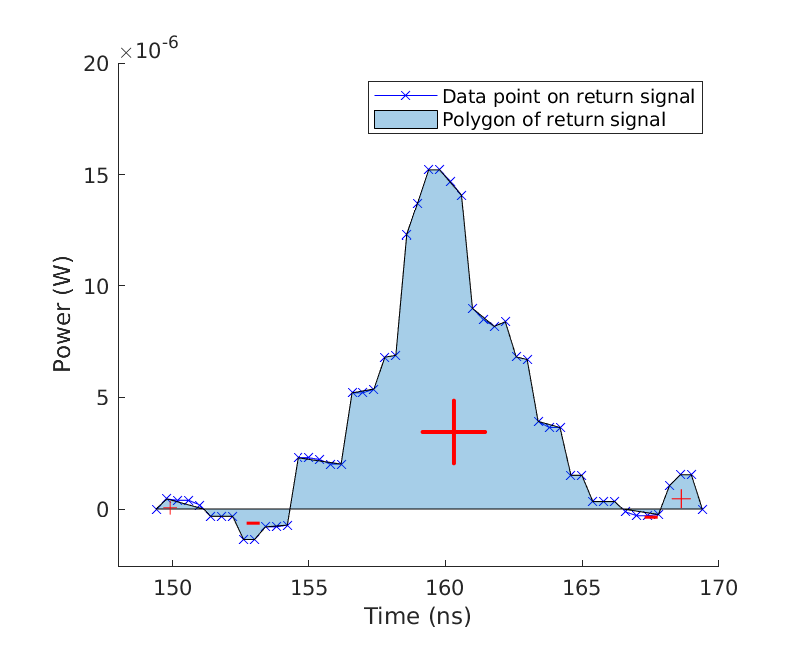
\includegraphics[width=0.8\textwidth]{figures/chapter6_ADC/polygon.eps}
\caption{Example of a polygon defined by data points of a return signal. Regions with '$+$' signs have positive area and regions with '$-$' sign have negative area.}
\label{fig:bm_polygon}
\end{figure}
The energy of the signal was approximated to be equal to the area of the polygon, which can be obtained numerically, by dividing the polygon into several triangles or rectangles and adding the area of each region together\citep{bourke1988calculating}. The mathematical expression is
\begin{equation}\label{eq:area} %% this equation is equivalent to the rieman sum
    A=\frac{1}{2}\sum\limits_{n=1}^{N}(t_nP_{r,n+1}-t_{n+1}P_{r,n}).
\end{equation}
where the $n$-th vertex of the polygon is denoted by $(t_n, P_{r,n})$ and $t_n$ and $P_{r,n}$ are the timestamp and the power value of the point, respectively. $N$ is the total number of data points in a signal. Since the power offset of the digital signal is removed by the ADC in advance, the power allows having negative values, which results in a self-crossing polygon, meaning the sides of the polygon intersect with itself. The negative values and the resultant negative areas of the self-intersecting polygon result in cancellation between the positive and negatives areas. The cancellation is consistent with our expectation that the energy of a signal having power with the same amplitudes but opposite signs is zero.\par
The peak power can be approximated by the \textit{y}-centroid $C_y$ of the polygon using
\begin{equation}\label{eq:bm_peakpower}
    P_{r,peak}=F_c\cdot C_y
\end{equation}
where $F_c$ is a constant factor and $F_c\approx3$. The value of $3$ is derived from combining Equation \eqref{eq:pulsemodel} and the fact that the height of a Gaussian pulse $h_{pulse}\approx2.828C_y$. The factor $F_c$ indicates that the peak power of a Gaussian pulse is always $F_c$ times the \textit{y}-centroid regardless of the signal amplitude. The constant relationship provides a more stable way of estimating the peak power than directly measuring the peak value of a pulse which is subject to large fluctuation due to the noise at the peak.\par
Applying the same approach in Equation \eqref{eq:area}, the centroid of the polygon can be obtained using the area $A$ by \citep{bourke1988calculating}:
\begin{align}
\label{eq:cen_x}
C_x=&\frac{1}{6A}\sum\limits_{n=1}^{N}(t_n+t_{n+1})(t_nP_{r,n+1}-x_{n+1}P_{r,n})\\
\label{eq:cen_y}
C_y=&\frac{1}{6A}\sum\limits_{n=1}^{N}(P_{r,n}+P_{r,n+1})(t_nP_{r,n+1}-x_{n+1}P_{r,n})
\end{align}
One should note that using Equation \eqref{eq:cen_x} and \eqref{eq:cen_y} on self-intersecting polygons will result in unexpected results \citep{bourke1988calculating}. Therefore, instead of using all the data points of a signal, only the points above zero are used for the centroid calculation. Also, to close a polygon the value of $P_{r, N+1}$ at $n=N$ is set equal to the value of $P_{r,1}$ in Equation \eqref{eq:area}, \eqref{eq:cen_x} and \eqref{eq:cen_y}, and to ensure the area cancellation, the value of $P_{r,N}$ and $P_{r,1}$ is set to zero, \ie $P_{r,1}=P_{r,N}=0$.\par
Now, given the energy $E$ and the centroid of the polygon $(C_x, C_y)$, the pulse width of a signal can be obtained by
\begin{equation}
    \Delta t_w = \frac{E}{F_c\cdot C_y}.
\end{equation}
%Estimation of arrival tim%
\subsection{Estimation of arrival time}
After the determination of the hypothesis of a signal, the arrival time of return pulses should be estimated. A simple way for the estimation is to use the timestamp of the peak of a pulse. However, the noise on the peak of a signal could impact the measurement accuracy and the result is also limited by the ADC resolution. Alternatively, we can approximate the lateral position of the peak by the \textit{x}-centroid of the signal, and use the timestamp of $C_x$ as the arrival time:
\begin{equation} \label{eq:bm_arrivalTime}
    t_{STOP}=C_x
\end{equation}
In this case, the resultant TOF and distance measurement is much less sensitive to the noise on the signal, and arrival time smaller than the ADC resolution can be resolved. To further improve the measurement accuracy, one can also use the data above the ADC threshold instead of the data above zero for Equation \eqref{eq:bm_arrivalTime}. It is because the data points above the threshold contain less noise than the data covering the whole noisy leading and falling edge. For a detailed discussion of using different data sets, please refer Section \ref{sec:bm_result}. One should note that the data above the threshold should not be used to calculate the \textit{y}-centroid of a signal, since the constant factor $F_c$ only holds for the data set that covers the entire curve of the Gaussian pulse.
%% Result 
\subsection{Results and discussion} \label{sec:bm_result}
Monte-Carlo experiment was performed on the benchmark detection and estimation algorithm using 500 observations of the return signals generated by the propagation and noise model. The tested SNR ranges from $60~dB$ to $8~dB$ (distance ranges from $2~m$ to $300~m$). Both edge and level trigger modes were tested. The settings of the trigger modes are given in Table~\ref{table:ADCtrigger}, in which $s$ is the number of bins that a signal contains above the ADC threshold and the value is depended on the signal amplitude. Also, the number of bins is set to be sufficiently large to cover the $1/e^2$ width of the Gaussian pulse. \todo{need to change post-cursor for edge (there is no post-cursor for edge)}
\begin{table}[h]
\centering 
\caption{Settings of ADC trigger modes}
\label{table:ADCtrigger}
\begin{tabular}{|l|c|c|c|c|c|}
\hline
Trigger mode            & \multicolumn{2}{c|}{Edge} & \multicolumn{3}{c|}{Level}                \\ \hline
Length of precursor ($bins$)        & $1$           & $1$           & $1$           & $2$            & $3$            \\ \hline
Collection-length($bins$) & $4$           & $5$           & \multicolumn{3}{c|}{$s$}                  \\ \hline
Length of post-cursor ($bins$)     & $1$           & $1$           & $1$           & $2$            & $3$            \\ \hline
Total length ($bins$)     & $6$           & $7$           & $2+s$       & $4+s$        & $8+s$        \\ \hline
Physical length ($ns$)    & $19.2$        & $22.4$        & $6.4+3.2s$ & $12.8+3.2s$ & $25.6+3.2s$ \\ \hline
\end{tabular}
\end{table}
%Result: pulse width%
\subsubsection{Pulse width measurement}
The pulse width of return signals with different SNRs was calculated and the results are given in Figure~\ref{fig:bm_pw}(a).
\begin{figure}[htbp] % position options
\centering
\graphicspath{ {figures/} }
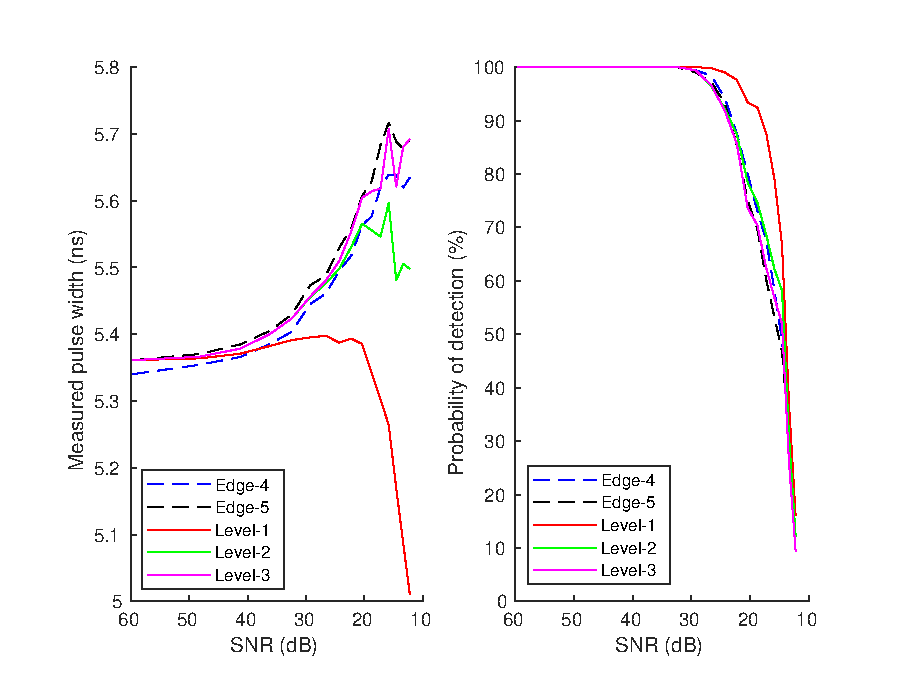
\includegraphics[width=0.8\textwidth]{figures/chapter6_ADC/pd_pw_snr_all.eps}
\caption{Pulse width measurement and Probability of detection}
\label{fig:bm_pw}
\end{figure}
In the figure, the number after the trigger mode indicates the collection-length in $bins$ for edge-triggering and the number of bins of precursor and post-cursor for level-triggering. The result shows that for a particular trigger setting the pulse width increases/decreases with the SNR, and at the same distance (SNR) the pulse width increases with the length (number of bins) of the signal. These trends apply to both edge-triggering and level-triggering. The reason for the trends is that the amplitude of the signal decreases with distance, and the edge-triggering samples a constant length of a signal. Therefore, a larger portion of the leading and falling edge of the signal was captured for a signal from a longer distance, which lowers the \textit{y}-centroid of the signal. Additionally, as the distance increases the leading and falling edge of the signal become noisier, and the noise contributes to a large area at the lower portion of the signal which reduces the \textit{y}-centroid. On the other hand, the measured area under the Gaussian curve remains almost constant as the positive and negative areas induced by the noise were canceled. Therefore, the pulse width increases according to Equation~\eqref{eq:bm_pw}, and more data points captured by the ADC give a longer pulse width. The same reason applies to the edge-triggering as well. Level-3 triggering that captures more data points gives a longer pulse width than the other two. Moreover, as the SNR decreases, the edges of a signal becomes noisier, which results in an increase of the pulse width for Level-2 and Level-3, respectively. An exception is Level-1, which captures the smallest portion of the edges. In this case, the effect of the noise on the pulse width is the minimum. However, on the other hand, the small size of the precursor and the post-cursor truncates the Gaussian pulse, which results in a rise of the \textit{y}-centroid of the signal and therefore, a smaller pulse width. \par
% One should note that even though the pulse width varies with SNR, the difference from  never exceeds the boundaries of the criterion ($$), and if the length of the precursor and post-cursor is selected properly, the pulse width could remain stable in a wide range of distance (Level-1). Moreover, when the SNR is less than $14~dB$, the number above threshold (Metric 1) becomes the decisive factor for the hypothesis determination rather than the pulse width. In other words, the value of pulse width has less effect on the signal determination.  we believe the pulse width metric is valid 
%%%Result: Pd and Pfa
\subsubsection{Probability of detection and  probability of false alarm}
The probability of detection and the probability of false alarm are normally used to evaluate the performance of a detector. The probability of detection is defined as the ratio of the number of signals detected as $\hone$ to the total number of $\hone$ signals, while the probability of false alarm is defined as the percentage of false-positive signals to the total number of noise signals. The probabilities of detection were calculated using the same return signals for the pulse width calculation, and the probabilities of false alarm at different trigger modes and ADC-trigger thresholds were computed using 500 noise signals generated by the noise model with laser pulse turned off. The results are shown in Figure~\ref{fig:bm_pw}(b). From the results we observe that the probability of detection remains greater than $99\%$ at a distance of $100~m$ with an SNR of $30~dB$. The corresponding largest pulse width among the trigger modes is $5.47~ns$ which 
is slightly larger than the upper limit of the criteria. Moreover, all the trigger modes give a probability of false alarm of zero for the ADC trigger at 3x the noise floor and $2\%$ for the trigger at 1x noise floor. Based on the probability of detection and false alarm, we conclude that the detection algorithm that uses the number above threshold and the pulse width of a signal as the metrics demonstrates a high performance on the signal detection for a target distance smaller than $100~m$ (SNR $>30~dB$). For a longer target distance (lower SNR), the increased pulse width reduces the probability of detection. However, if the trigger mode and the length of the precursor and post-cursor is selected properly (\eg Level-1), the distance can be extended to $150~m$ ($23~dB$) with a probability of detection of $99\%$ and $200~m$($19~dB$) with the probability of $92\%$.
% even though the variation of the pulse width at different trigger settings reduces the probability of detection when the SNR decreases, but note that when the SNR is less than $14~dB$ Metric 1 becomes the decisive factor for the hypothesis determination rather than the pulse width.. Consequently, according to the high probability of detection and low false alarm rate at the long distance, we can see the benchmark detection algorithm using the NaT and pulse width gives a good performance of signal detection at least for the distance smaller than $260~m$ (SNR $>14.57~dB$).
%%% Result: Accuracy
\subsubsection{Accuracy and RMS error of distance measurement}
The accuracy (mean error) and the RMS error of the distance measurement using the benchmark estimation algorithm are also evaluated on the 500 observations of the return signal at different distances using both edge and level triggering. The mean error $\overline{\Delta d}$ and the RMS error $\sigma_d$ are defined as
\begin{align}
\overline{\Delta d} = \frac{1}{M}\sum_{m=1}^{M}(d_{meas,m} - d_{GT})\\
\sigma_d = \sqrt{\frac{1}{M}\sum_{m=1}^{M}(d_{meas, m}-\overline{d_{meas}})^2}
\end{align}
where $d_{meas, m}$ is the distance measurement of the $m$-th observation of the total $M$ observations, after converting the measured TOF to distance. $\overline{d_{meas}}$ is the average distance measurement over the $M$ observations for a certain distance and $d_{GT}$ is the corresponding ground-truth distance. The results of the errors are shown in Figure~\ref{fig:bm_error_edge} and Figure~\ref{fig:bm_error_level}.
\begin{figure}[t!p]
\centering
\graphicspath{{figures/}}
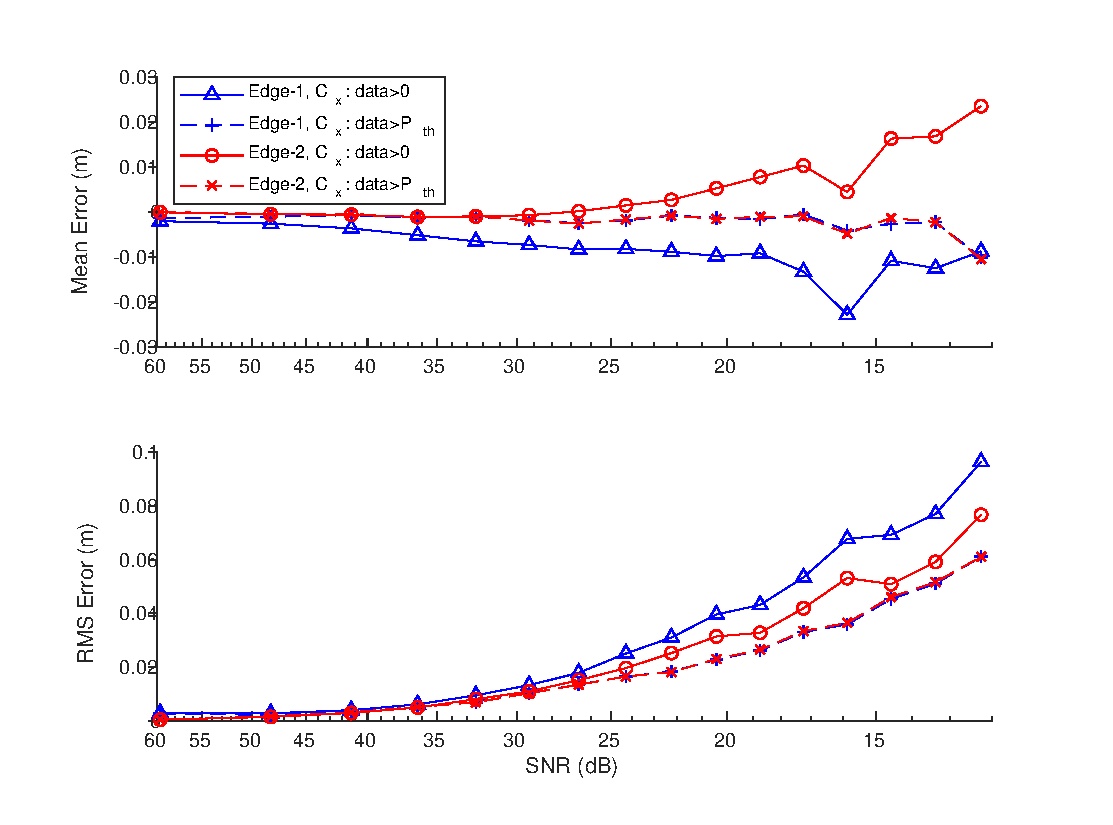
\includegraphics[width=.8\textwidth]{figures/chapter6_ADC/error_snr_edge.eps}
\caption{Mean error and RMS error of distance measurement using edge triggering: edge-1 and edge-2. Distance calculated using data greater than zero is shown in solid lines and using data greater than the ADC threshold is shown in dashed lines.}
\label{fig:bm_error_edge}
\end{figure}%
\begin{figure}[t!p]
\centering
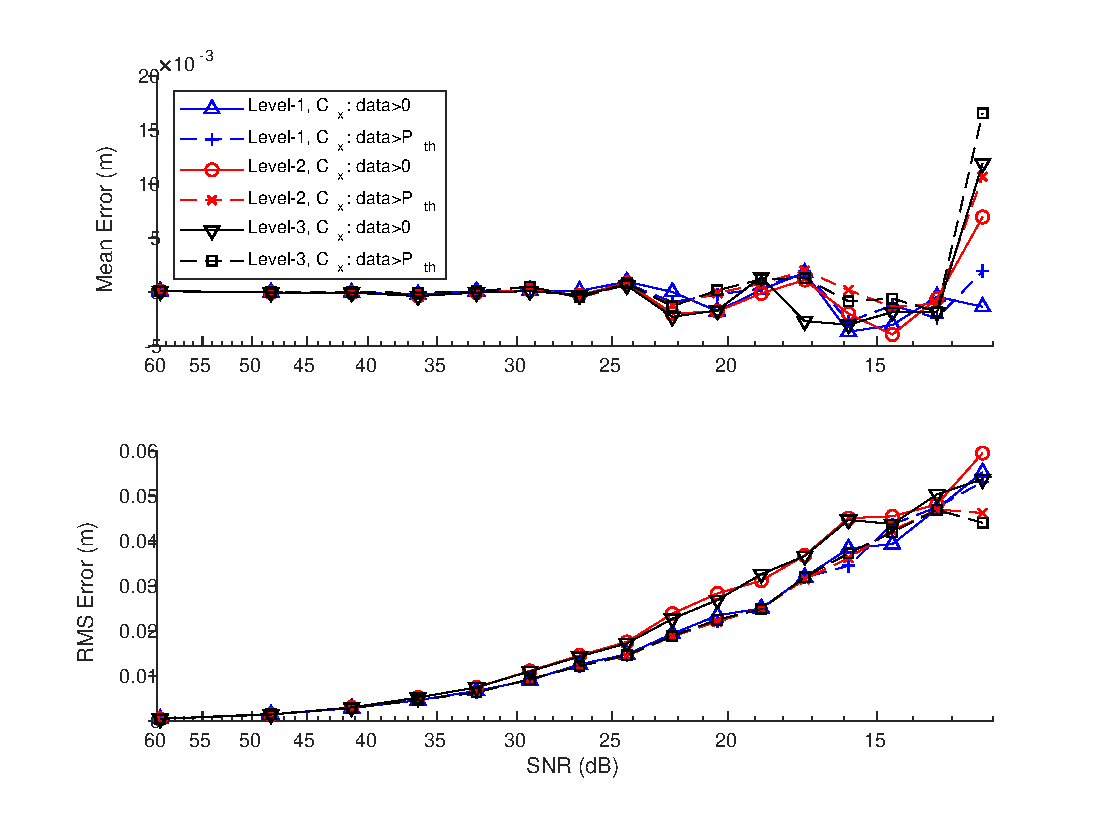
\includegraphics[width=.8\textwidth]{figures/chapter6_ADC/error_snr_level.eps}
\caption{Mean error and RMS error of distance measurement using level triggering: level-1, level-2, and level-3. Distance calculated using data greater than zero is shown in solid lines and using data greater than the ADC threshold is shown in dashed lines.}
\label{fig:bm_error_level}
\end{figure}
%%%
\begin{figure}[t!p] % position options
\graphicspath{ {figures/} }
\centering
    \begin{subfigure}{.7\textwidth}
    \centering
    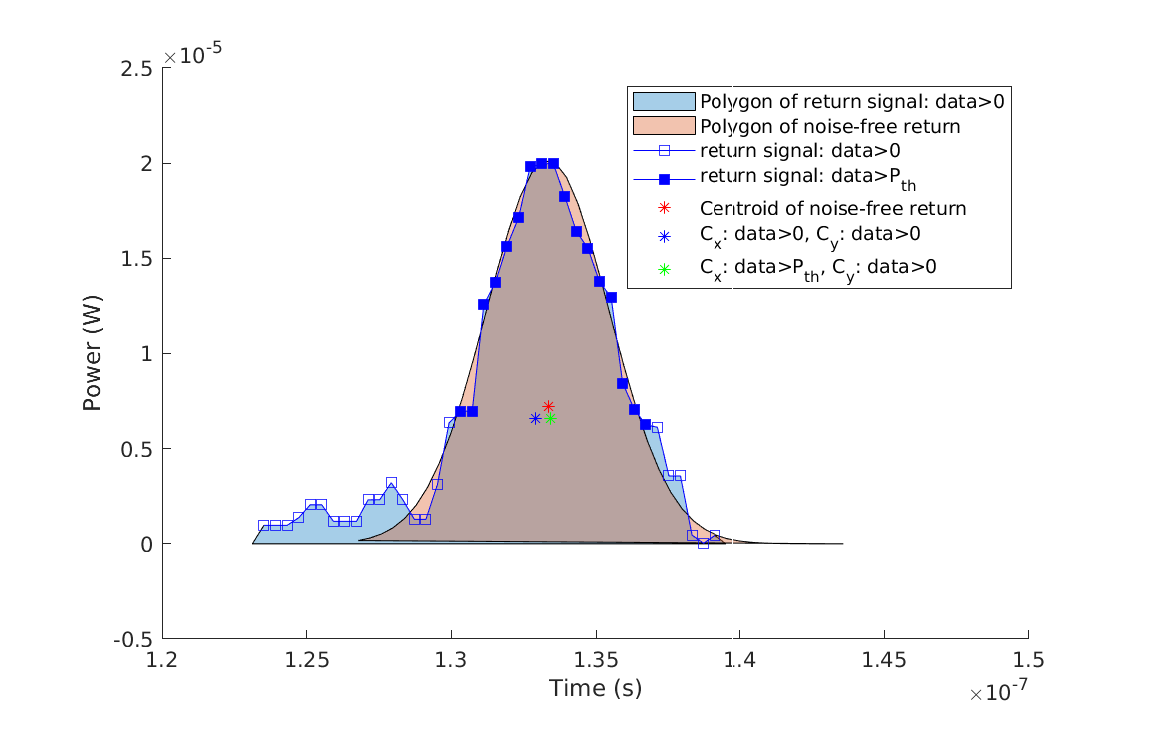
\includegraphics[width=.8\textwidth]{figures/chapter6_ADC/centroid_edge1_d_20_snr20_41.eps}
    % \label{fig:bm_leftshift_edge1}
    \end{subfigure}%
    
    \begin{subfigure}{.7\textwidth}
    \centering
    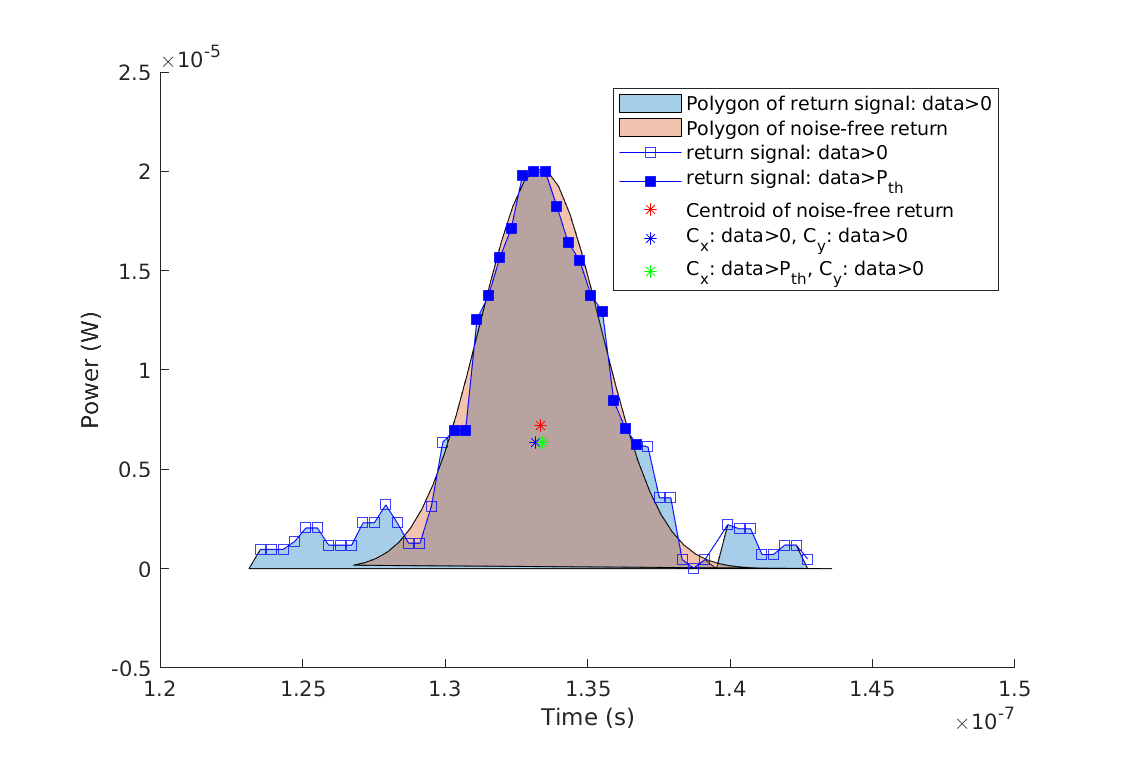
\includegraphics[width=.8\textwidth]{figures/chapter6_ADC/centroid_edge2_d_20_snr20_41.eps}
    % \label{fig:bm_leftshift_edge2}
    \end{subfigure}%
    
    \begin{subfigure}{.7\textwidth}
    \centering
    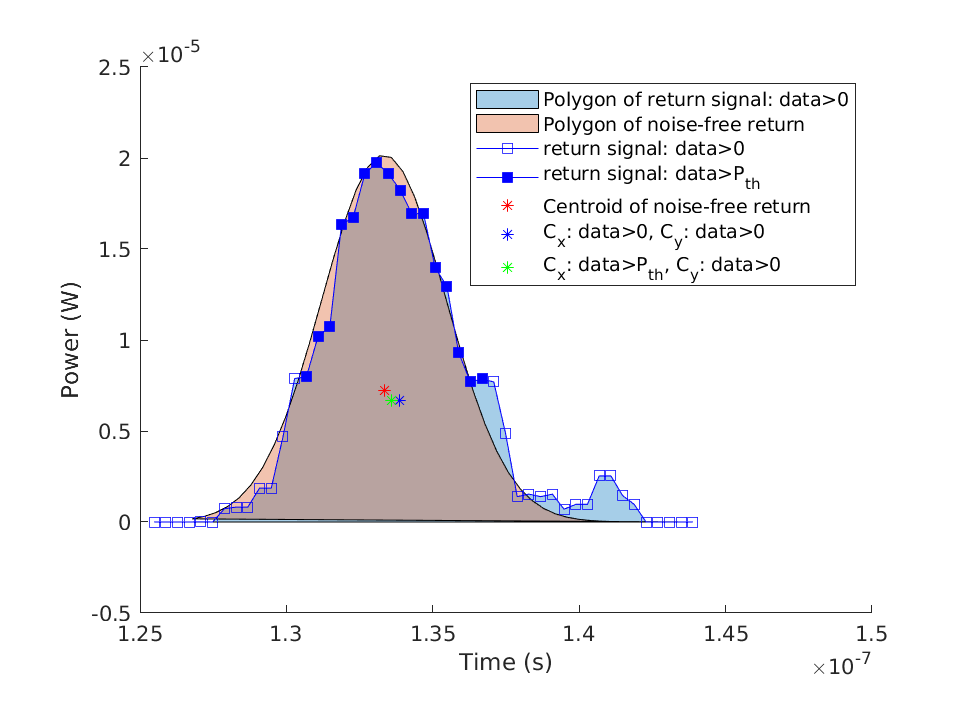
\includegraphics[width=.8\textwidth]{figures/chapter6_ADC/centroid_edge2_d_20_snr20_41_id131.eps}
    % \label{fig:bm_rightshift_edge2}
    \end{subfigure}
    \caption{(a) Left-shift, (b) non-shift (c) right-shift of the \textit{x}-centroid. Case (a) and (b) use the same signal with different trigger settings and Case (c) uses a different signal. The SNR of the signals at all the cases is $20.41~dB$. The trigger settings are (a) Edge-1 (b) Edge-2 and (c) Edge-2.}
     \label{fig:bm_shift}
\end{figure}
From the results, we notice that the mean distance error for the edge triggering using data above zero presents a negative or positive bias. The reason is that at a low SNR the noise on the signal could cause an early triggering on the signal and since the edge-triggering samples a constant length of a signal, a longer leading edge and a shorter falling edge of the signal are captured. The asymmetric signal \wrt the vertical center line of the Gaussian pulse causes the left-shift of the \texttt{x}-centroid and consequently, an earlier arrival time and shorter target distance. Figure~\ref{fig:bm_shift}(a) illustrates the left-shift of the \textit{x}-centroid of the signal. In the figure, the blue star stands for the \textit{x}-centroid using data greater than zero and the red star represents the \textit{x}-centroid of a corresponding noise-free signal. The blue star is shift left to the red star because of the larger portion of leading-edge included in the signal. Setting a longer length of the precursor and post-cursor to cover a longer falling edge could partially reduce the left-shift. An example is shown in Figure~\ref{fig:bm_shift}(b), in which the same signal is sampled by twice the length of the precursor and post-cursor used in Figure~\ref{fig:bm_shift}(a). In this case, the blue star moves closer to the red star. However, since the trigger position on the signal is random and difficult to predict, a longer falling edge could also cause a right-shift of the \textit{x}-centroid and a further target distance (red solid line in Figure~\ref{fig:bm_error_edge} (a)). An example of the right shift of the \textit{x}-centroid is provided in Figure~\ref{fig:bm_shift}(b), in which the blue star shifts to the right of the red star because of the longer falling-edge captured by the ADC.\todo{label figure}\par
Adjusting the length of the precursor and the post-cursor of the edge-trigger is not an optimal solution to the negative/positive bias of the distance measurement due to the randomness of noise. An alternative solution is to use the data above the ADC threshold rather than the data greater than zero. The benefit of using those data points is that most of the data points above the threshold are belong to the Gaussian pulse instead of noise and they have symmetrical distribution around the vertical center line of the pulse. In this case, the \textit{x}-centroid is calculated from symmetric signals. The results of using data above the threshold are shown in the dashed lines in Figure~\ref{fig:bm_error_edge}, which presents a much less bias than the results using the data points above zero. Contrary to the edge-triggering, the positive/negative bias does not appear on the results of level-triggering (Figure~\ref{fig:bm_error_level}(b)). This is because the nature of the level-triggering is to capture the data points above the threshold and symmetric signals are captured for the \textit{x}-centroid calculation.\par
From the results of the RMS error (Figure~\ref{fig:bm_error_edge}(b) and Figure~\ref{fig:bm_error_level}(b)), we can see that for the edge-triggering, covering a larger portion of the pulse balances the fluctuation of the measurement caused by the noise at the leading and falling edge of the signal and yielded a smaller RMS error. However, the length should be chosen with cautions to avoid positive or negative bias on the distance measurement. On the contrary, a smaller size of the precursor and post-cursor for the level-triggering reduces the effect of noise on the centroid measurement and improves the measurement accuracy. The RMS error using data greater than zero and data above the ADC threshold are also compared, and the former one gives a larger RMS error, which is because the noise included in the signal causes a larger fluctuation that the later one on the \textit{x}-centroid measurement and the distance measurement.


% suggestoni: capture large enough portion of the gaussian shape, but least noise


% result1: accuracy and std, pd vs SNR for edge, level-8 and level-16.
% discussion on accuracy (level and edge) : left and right shift
% discussion on pd: how # and pd changes with SNR, show polygon plots.

% results 2: after AFE, check how pw changes
% results 3: different kind noises
% pw variance with SNR
% error vs SNR, pfa and pd vs SNR, ROC, 
% different noises on error, pfa, pd ...
% measurements on real data

